\chapter{Verification, Security Testing, Limitations, and Future Work}
\thispagestyle{plain}
\section*{Introduction}
\addcontentsline{toc}{section}{Introduction}
This chapter evaluates the platform from the perspective of software assurance and operational maturity. It explains the real verification layers present in the repository, the gaps that remain, the security implications of current deployment choices, and the most credible next steps.

\section{Verification as an Engineering Discipline}
Verification should not be reduced to the question of whether unit tests exist. In software engineering, verification encompasses every mechanism used to establish that the implemented system conforms sufficiently to its intended behaviour, while validation addresses whether the right system was built for the problem at hand. Security platforms complicate this distinction because correctness is rarely exhausted by pure function-level logic. A system may be locally correct in code yet operationally weak if its deployment, trust boundaries, fallback behaviour, or failure visibility are poorly controlled.

For that reason, this chapter evaluates the platform across several verification layers: static correctness, runtime integration confidence, user-interface walkthroughs, security control review, and operational maturity. This broader view is necessary because the project's strongest properties are not located only in unit-level logic; they are also visible in its architecture, operator workflows, and degradation behaviour.

\section{Testing Strategy Overview}
The testing posture of the project must be described honestly. The repository does not contain a broad conventional unit and integration test suite. Instead, verification is weighted toward static analysis, smoke testing, manual end-to-end validation, and browser-driven walkthroughs. This is weaker than a mature CI-backed engineering baseline, but stronger than an unvalidated prototype.

This shape can be interpreted through the idea of a practical rather than idealized test pyramid. In a textbook pyramid, unit tests are numerous, integration tests fewer, and end-to-end tests relatively sparse. The project departs from that ideal because it was developed under tight scope and because many of its highest-risk behaviours lie at service boundaries, not only in pure internal functions. The resulting profile is therefore closer to an ``inverted'' or boundary-heavy strategy, where broad unit coverage is missing but real-stack and UI-level verification remain meaningful.

\begin{figure}[H]
\centering
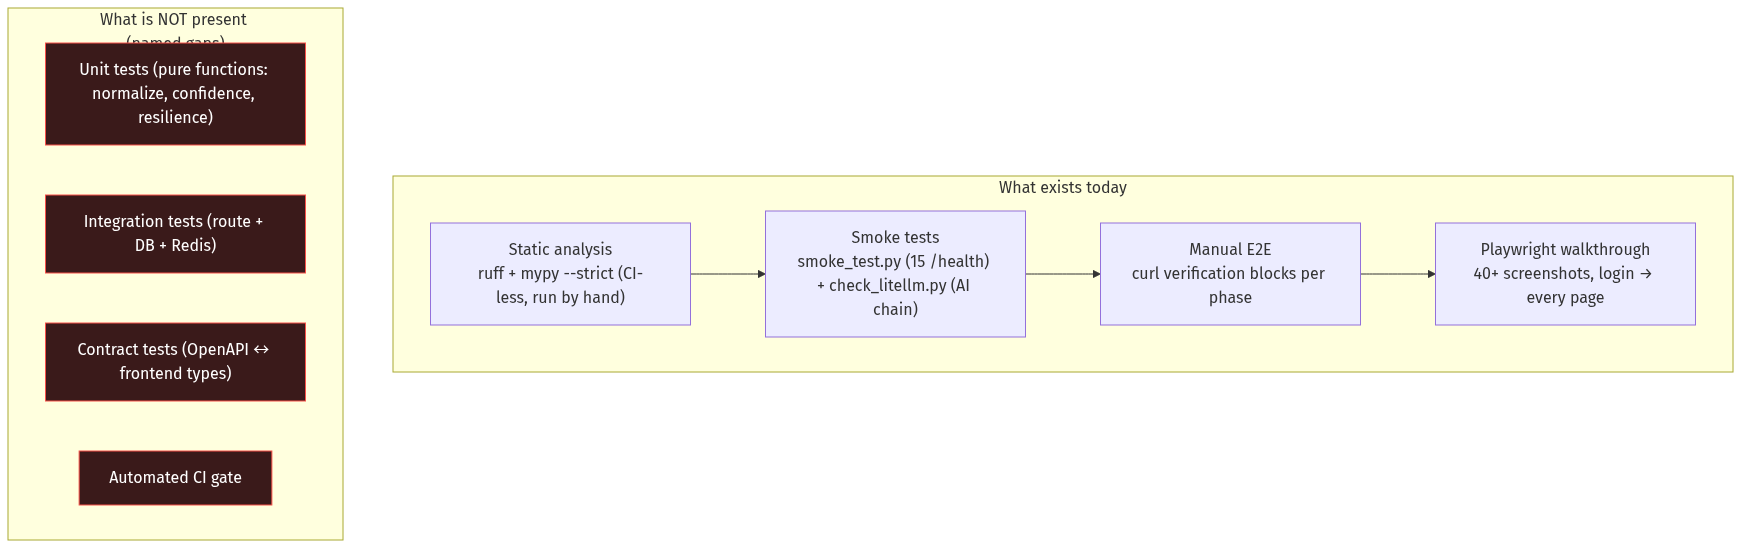
\includegraphics[width=0.85\textwidth]{images/tip/diagrams/11_test_strategy.png}
\caption{Verification strategy used by the project.}
\label{fig:test-strategy-new}
\end{figure}

\section{Unit Testing}
\subsection{Current State}
There is no substantive first-party unit test suite across the services and shared packages. This is an architectural and process limitation, not something that should be reframed as a hidden strength.

\subsection{What Is Indirectly Covered}
Some of the logic that would normally be exercised through unit tests is instead protected by static typing, validation models, and shared abstractions. The strict MyPy configuration and Ruff checks reduce type-level and API-shape regressions. Pydantic models catch many malformed inputs and schema mismatches. Shared helper functions reduce the amount of per-service duplicated logic that would otherwise need isolated tests.

Static analysis has particular value in this codebase because much of the platform's complexity lies in contract surfaces: typed settings, request and response schemas, service dependencies, and structured AI outputs. Type errors, shape mismatches, and inconsistent signatures are therefore not superficial issues. They are a large class of real defects that static tools can catch before runtime. This does not replace unit testing, but it does explain why static checks provide more defensive value here than they would in a loosely typed scripting codebase.

\subsection{What Should Be Unit Tested First}
If a unit test layer were added, the highest-value targets are clear: indicator normalization, confidence-score calculation, permission matching, scheduler callback helpers, secrets client fallback behaviour, AI response-shape validation, and risk or prioritization helpers that operate as pure logic.

\section{Integration Testing}
\subsection{Current State}
There is no broad automated integration suite that programmatically brings services together and validates inter-service contracts in a repeatable harness.

\subsection{What Exists Instead}
In practice, the repository relies on live-stack verification. Compose is used to stand up the full environment, migration and seed scripts create a usable state, and smoke tests verify service reachability. This approach gives higher-fidelity feedback on infrastructure wiring and service bootstrap, but weaker repeatability and lower isolation than a formal integration suite.

The theoretical strength of live-stack validation is environmental realism. It exercises the actual database, pooler, cache, container startup order, secret bootstrap, and inter-service routing topology. Its main weakness is reproducibility and automation depth. In other words, it is strong at catching integration reality and weak at supporting cheap regression frequency. That distinction is important because it shows the current verification posture is incomplete, not absent.

\section{End-to-End Testing with Playwright and Manual Walkthroughs}
The frontend and operational workflows are better covered than the backend unit layer. The repository contains a browser-driven walkthrough process that captures the UI surface and validates page-level navigation and rendering. The screenshots preserved in the LaTeX project are direct evidence of that process.

This style of validation is particularly useful for the frontend because the application depends on a BFF proxy, permission-sensitive navigation, authentication state, and cross-service aggregation routes. A narrow backend-only test would not catch many of the failure modes visible at the application boundary.

There is also a methodological point here. In systems where the frontend is a real integration boundary rather than a static veneer, browser-driven validation becomes more than cosmetic testing. It checks assumptions about authentication persistence, route aggregation, permission-gated navigation, latency tolerance, and the practical readability of outputs. Those are all part of system quality for an analyst-facing platform.

\section{Security Testing and Security Validation}
\subsection{Input and Schema Validation}
Request validation is strongly supported through FastAPI and Pydantic schemas. This gives consistent request-body parsing, query validation, and response typing across services.

\subsection{Authorization Validation}
Authorization intent is explicit in route dependencies. This makes missing permission checks visible in code review, even if the current deployment relaxes enforcement for many internal services.

\subsection{OWASP-Relevant Controls}
The platform implements several controls aligned with common web and API security guidance: role-based permissions, hashed passwords, hashed refresh tokens, centralized secrets, limited secret exposure through metadata-only listing, validation-driven request handling, and separation of public and bootstrap-only secret flows. However, the platform also carries real security debt: internal service auth is relaxed in Compose, provider access is centralized but still dependent on bootstrap secrets, and some backend ports are exposed directly.

Security verification in this context is therefore partly structural. Some claims can be supported by direct implementation evidence: passwords are hashed, refresh tokens are not stored in the clear, route dependencies make authorization intent visible, and secrets are centralized. Other claims require the opposite posture: they must be explicitly withheld because the implementation does not support them. This is why the thesis must discuss the softer internal trust boundary candidly rather than implying stronger guarantees than the runtime configuration actually provides.

\section{Performance Testing and Benchmarking}
There is no formal load-testing or benchmarking suite in the repository. Performance claims therefore need to remain bounded and honest. The strongest supported claim is architectural rather than numerical: the platform optimizes the hot IOC path, caches AI outputs to control cost and latency, uses PgBouncer to limit database pressure, and keeps ingest off the AI path so data freshness is not coupled to inference performance.

This chapter should therefore distinguish between performance design and performance proof. The repository clearly contains performance-aware design: hot-path caching, pooled connections, controlled fan-out, and bounded AI usage. What it does not yet contain is a formal measurement programme capable of turning those design intentions into rigorous throughput and latency claims. That gap belongs to future work, not to the current claim set.

\section{Verification Flow in Practice}
The de facto acceptance flow for changes is shown in Figures~\ref{fig:verify-new} and \ref{fig:verify-bottom}.

\begin{figure}[H]
\centering
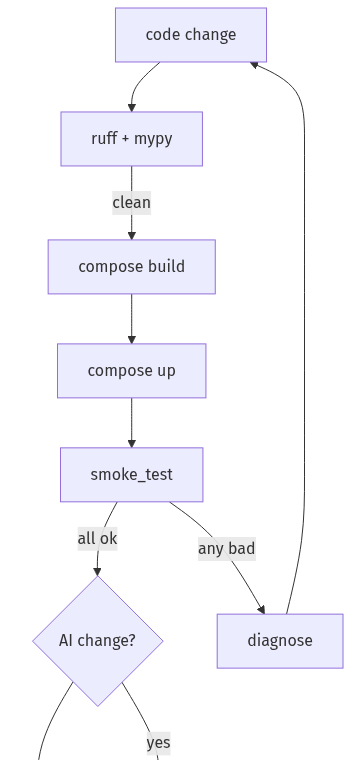
\includegraphics[width=0.5\textwidth]{images/tip/diagrams/11_verification_flow_top.png}
\caption{Manual verification flow used before accepting changes, upper segment.}
\label{fig:verify-new}
\end{figure}

\begin{figure}[H]
\centering
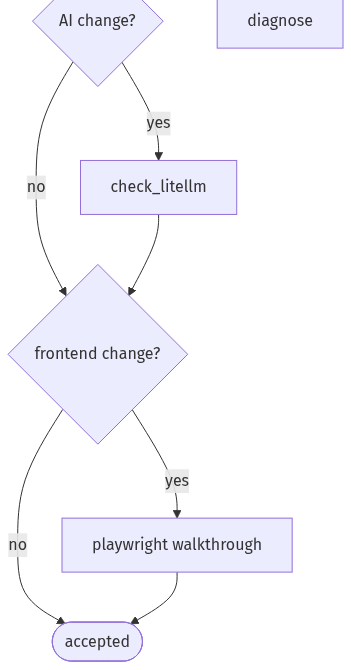
\includegraphics[width=0.5\textwidth]{images/tip/diagrams/11_verification_flow_bottom.png}
\caption{Manual verification flow used before accepting changes, lower segment.}
\label{fig:verify-bottom}
\end{figure}

This process is manual rather than CI-driven, but it is coherent. Static checks run first, followed by rebuild and recreate of impacted services, smoke testing, AI-chain testing when relevant, and browser walkthroughs for user-visible changes.

\section{Key Limitations}
\subsection{Testing Maturity}
The largest engineering gap is the absence of a broad automated unit and integration suite. The platform has meaningful verification, but it does not have the regression depth expected of a production-hardened multi-service system.

\subsection{Operational Hardening}
The platform runs on one host and does not yet implement an automated backup and recovery regime, formal CI/CD, or a richer metrics-and-alerting pipeline. These are classic day-two maturity gaps.

\subsection{Security Boundary Simplification}
Inter-service authentication is relaxed behind the Docker network for most services. This simplifies operation and avoids some service-to-service failure modes, but it creates a softer internal trust boundary than a stricter zero-trust design would provide.

\subsection{AI Dependence and Quota Sensitivity}
AI features are intentionally separated from ingestion, but the analytical layer remains dependent on external model providers and their quotas. The platform mitigates this through caching, fallback chains, and persistent output materialization, yet it does not eliminate the dependency.

Taken together, these limitations reveal a consistent maturity profile. The platform is relatively strong on domain modelling, service structure, contextual intelligence workflows, and bounded AI integration. It is weaker on automation depth, infrastructure redundancy, and formally measured non-functional proof. That is a normal profile for a successful PFE-scale engineering artefact, but it should remain explicit so the reader understands where the contribution genuinely lies.

\section{Future Work}
The most credible next steps are incremental rather than architectural rewrites.

\subsection{Testing Roadmap}
The highest-value improvement is to add unit tests around pure logic and integration tests around the most security-sensitive service boundaries, especially auth, secrets, scheduler callbacks, and orchestrator reporting.

\subsection{Operational Hardening}
Automated database backups, restore drills, CI/CD gates, and metrics-backed alerting should follow soon after. These changes improve reliability without requiring a fundamental redesign.

\subsection{Security Hardening}
A production-grade evolution of the platform should re-enable and validate inter-service auth selectively, reduce direct exposure of non-frontend service ports, and strengthen bootstrap-token handling and rotation.

\subsection{Scalability Evolution}
The schema-per-service design and explicit service URLs make it feasible to move the heaviest services or stores onto separate hosts later, but that should follow operational hardening rather than precede it.

\chapter*{General Conclusion}
\addcontentsline{toc}{chapter}{General Conclusion}
The implemented Threat Intelligence Platform responds to a concrete operational problem: a security team working under modern threat pressure cannot afford to manually assemble context from disconnected feeds, vulnerability sources, indicator stores, actor libraries, and internal tooling every time it needs to make a triage or prioritization decision. The system addresses that problem by combining continuous ingestion, deterministic normalization, organization-aware prioritization, structured AI-assisted synthesis, and a user interface that makes those outputs operationally usable.

From an architectural perspective, the strongest aspects of the platform are its disciplined service ownership model, its clear separation between ingest and synthesis, its shared service skeleton, its centralized secret handling, and its practical use of a BFF proxy and scheduler control plane. From an operational perspective, its main value lies in turning raw threat information into a ranked and contextualized decision surface without forcing the team to depend on many separate tools.

The platform is also notable for what it does not pretend to be. It is not yet a highly available distributed system. It does not have mature automated test depth. It does not claim strict zero-trust internal segmentation in its current Compose deployment. These are real limitations, but they do not undermine the core contribution of the work. They show that the system is a technically coherent and operationally credible platform whose remaining gaps lie mainly in hardening, automation, and production engineering maturity rather than in basic design.

The most important result is therefore not only that the platform works, but that its internal structure makes improvement tractable. Testing can be deepened without redesign. Stronger service-to-service auth can be reintroduced without abandoning the current service model. Operational safeguards such as backup automation, CI/CD, and richer observability can be added incrementally. That combination of functional completeness, explicit tradeoffs, and credible upgrade paths is what makes the system thesis-worthy as an engineering artefact.
